\chapter{Manuel de jeu}
\section{Jouer une partie}
Lorsque vous rentrez en jeu, les joueurs et les balles sont placés à leur position initiale. Chaque type de joueur est identifié par une couleur: \textbf{bleu} pour les \gls{chaser}s, \textbf{rouge} pour les \gls{beater}s, \textbf{vert} pour le \gls{keeper} et \textbf{jaune} pour le \gls{seeker}. Les joueurs aux costumes rayés sont ceux de votre adversaire, les vôtres sont en couleurs pleines.

\subsection{Sélection d'un joueur}
\begin{figure}[h!]
    \centering
    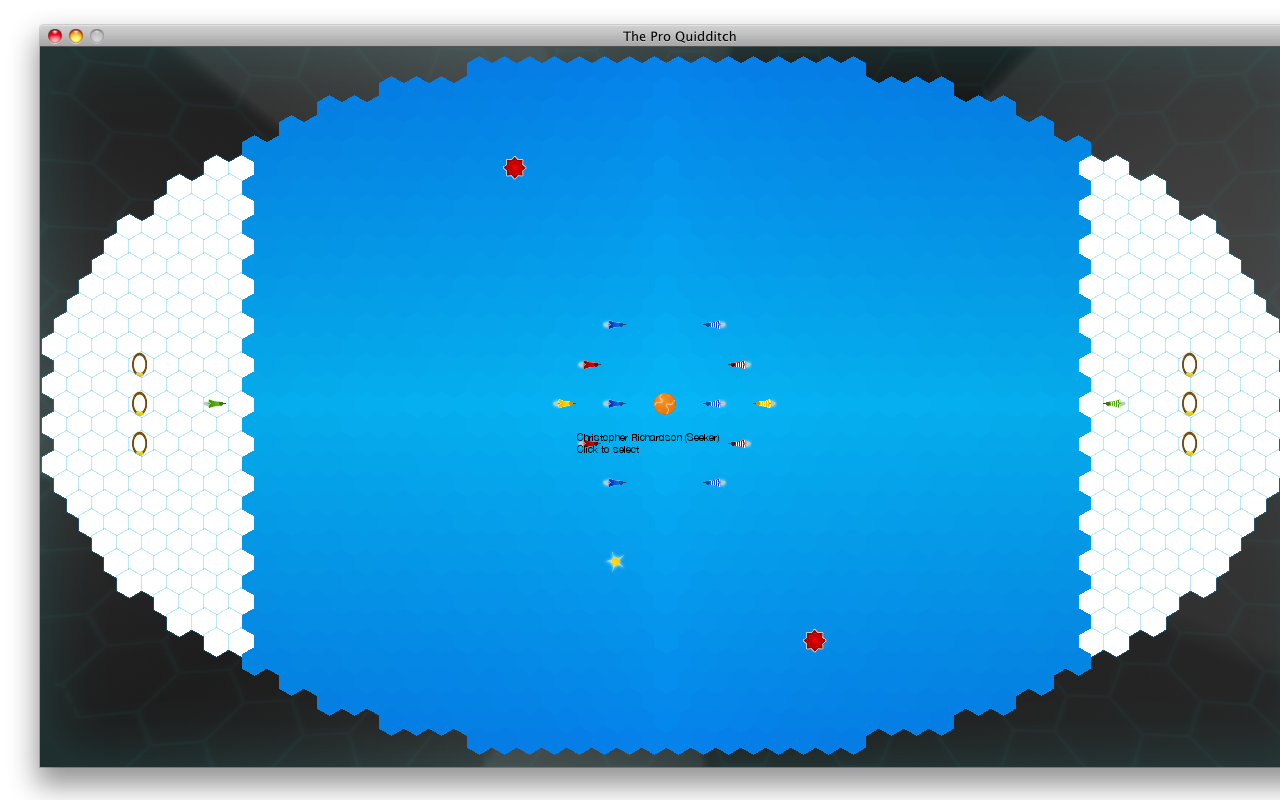
\includegraphics[width=\textwidth]{../screenshots/hover_seeker.png}
    \caption{\label{manual:view_name} Affichage du nom de l'attrapeur lorsque la souris le survole}
\end{figure}

Passez votre souris sur les joueurs pour découvrir leur nom (voir figure \ref{manual:view_name}). Comme l'outil d'aide le suggère, vous pouvez cliquer dessus pour les sélectionner. Une fois votre joueur sélectionné, les cases qu'il peut atteindre sont mises en évidence en jaune. Cliquez sur l'une d'elle: le chemin que parcourera votre joueur est affiché en rouge (voir figure \ref{manual:assign_move}). S'il peut encore continuer, les prochaines cases sont à nouveau mises en évidence en rouge. Pour terminer le mouvement d'un joueur, re-cliquez sur la dernière case atteinte.

\begin{figure}[h!]
    \centering
    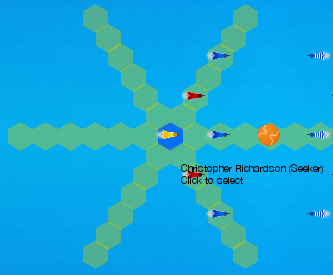
\includegraphics[width=0.5\textwidth]{../screenshots/assign_move.png}
    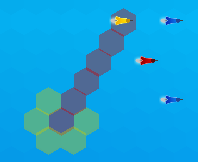
\includegraphics[width=0.5\textwidth]{../screenshots/assign_move2.png}
    \caption{\label{manual:assign_move} Affichage des cases atteignables par un joueur}
\end{figure}

\subsection{Actionner une balle}
Certains joueurs peuvent utiliser des balles. Les 
